\section{Prototype interviews}\label{section:interview2}
State of The Art undersøgelsen viste at der er mange forskellige løsninger, men der er også mange mangler i disse alligevel.
Ingen af løsningerne tager tilbud fra alle butikker, har indkøbsliste, tilbyder opskrifter der er integreret med tilbudene, samt vurdering af disse.
Løsningerne
Derfor har vi udformet en prototype i Microsoft Office Powerpoint som viser forskellige funktionaliteter.
Diasshowet består af forskellige skærmbilleder, som der kan navigeres imellem ved tryk på de gule felter.

Et eksempel kan ses på \myref{ss:Prototype}.

\begin{wrapfigure}{o}{0.68\textwidth}
\vspace{-20pt}
	\begin{center}
		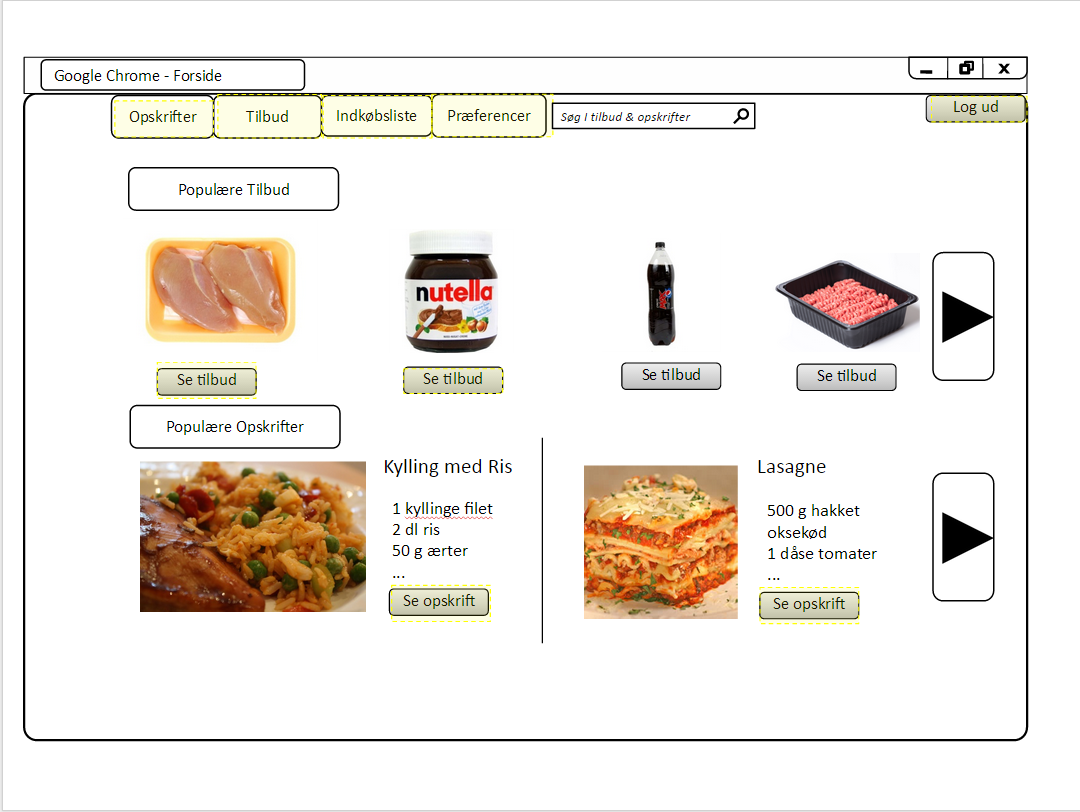
\includegraphics[width=0.66\textwidth]{images/Images/prototype-forside.PNG}
	\end{center}
	\vspace{-20pt}
	\caption{Forside fra Prototypen, der blev brugt i forbindelse med vores 2. runde af interviews}\label{ss:Prototype}
	\vspace{-20pt}
\end{wrapfigure}

Prototypen bruges i vores 2. runde af interviews, som har til formål at forstå hvilke funktionaliteter potentielle brugere ønsker i en løsning.
Den tidligere interviewrunde resulterede i et grundlag for en målgruppe, som følge af den, bestod de interviewede mest af unge personer i starten af tyverne, hvor af de fleste var studerende såvel som en repræsentant for de ældre.
Dette valg blev taget da ud fra det første interview, hvor den primære interesse lå hos de unge, der i forvejen brugte deres smartphone og computer til planlægning af indkøb og aftensmad.
Således ville en overgang til en ny løsning her være mere naturlig end de ældre grupper, der ofte laver listen på papir og har bøger med opskrifter til at finde inspiration.
På trods af dette var der stadig en interesse i den ældre gruppe, og målgruppen er som følge deraf ikke udelukkende unge.

Den 2. runde af interviews blev udført som semi-struktureret interviews, med personer hvor der var oprettet kontakt på forhånd, frem for at finde fremmed på gaden.
Dette tillod os at interviewe i længere tid, såvel som at de interviewede i forvejen var forberedt på et interview.
Et semi-struktureret interview tillader at der afviges fra de nedskrevne spørgsmål, for at følge samtalen og stille uddybende spørgsmål omkring potentielle kommentare.\fxnote{Find eventuel kilde fra DEB? - Marc}

De spørgsmål, som de adspurgte blev præsenteret for, var lavet med den præmis at få deres tanker omkring et system, inden de blev repræsenteret for de idéer der ellers var omkring systemet.
For at opnå dette, blev de først spurgt om et spørgsmål som hvilke opgaver de mente systemet kunne behjælpe, hvorefter der blev uddybet hvorfor præcis disse funktionaliteter blev nævnt af de interviewede.
Først efter at have fået deres idéer, blev de repræsenteret for idéer projektgruppen havde opnået, og herefter reflekteret over hvorfor nogle ikke var nævnt, smat hvad de mente om disse forslag.
Et dokument over de strukturerede spørgsmål af interview-sessionerne, kan findes på \myref{ch:PrototypeInterview}%Interview2.
Ud fra den respons der blev opnået igennem undersøgelsen, står det klart at en løsning skal have følgende funktionaliteter:

\begin{itemize}
	\item Indkøbsliste integreret med tilbud.
	\item Oversigt over tilbud fra samtlige dagligvarebutikker.
	\item Opskrifter, som gør brug af tilbud.
	\item Mulighed for at vurdere opskrifterne og få anbefalet lignende.
	\item Valg af hvor man vil handle, hvilke madvarer man ikke vil spise osv.
	\item Deling af indkøbsliste med andre.
	\item Filtrering under opskrifter, så man kan se hvad man kan lave ud af f.eks. oksekød osv.
	\item Overvågning af varer, så man får en form for besked hvis noget kommer på tilbud en uge.
\end{itemize}

Der var også andre funktionaliteter som nogle af de adspurgte foreslog kunne laves for systemet, disse er dog blevet fravalgt, enten fordi det kun var enkelte der bakkede op omkring den funktion, eller at det ikke passede ind med systemets anden funktionalitet.
F.eks. blev en kalorietæller foreslået af en af de adspurgte, men dette vælges der at afgrænses fra, da det ikke hænger så godt sammen med resten af den meget tilbudsorienterede løsning.

Herudover gav de interviewende også forslag og råd angående hvilke funktionaliteter skulle være hvor i et desktop layout.
Disse forslag tages med i overvejelserne når brugergrænsefladen skal designes.
En oversigt over de adspurgtes svar såvel som forslag, kan ses på \myref{ch:protorespons}%Interview2 Opsummering
